%%%%%%%%%%%%%%%%%%%%%%%%%%%%%%%%%%%%%%%%%%%%%%%%%%
\documentclass[12pt]{article}
\usepackage{epsfig,verbatim}
\usepackage{color}
%\pagestyle{headings}
\textheight 8.5 in
\textwidth 6.5 in
\topmargin -0.35 in
%\topmargin -0.10 in
\oddsidemargin -0.1 in
\renewcommand{\topfraction}{1}
\renewcommand{\bottomfraction}{1}
\renewcommand{\textfraction}{0}
\renewcommand{\floatpagefraction}{0.90}
\makeatletter
\def\singlespace{\def\baselinestretch{1}\@normalsize}
\def\endsinglespace{}
\newtheorem{lemma}{Lemma}%[section]
\newtheorem{theorem}{Theorem}%[section]
\newtheorem{remark}{Remark}
\newtheorem{example}{Example}%[section]
\newtheorem{corollary}{Corollary}%[section]
\@addtoreset{equation}{section}
\renewcommand{\theequation}{\thesection.\arabic{equation}}
\renewcommand{\thefootnote}{\fnsymbol{footnote}}
\renewcommand{\hat}{\widehat}
\def\singlespace{\def\baselinestretch{1}\@normalsize}
\def\endsinglespace{}
\makeatother
\def\c{\centerline}
\newcommand{\by}{\mbox{\bf y}}
\newcommand{\bX}{\mbox{\bf X}}
\newcommand{\bZ}{\mbox{\bf Z}}
\newcommand{\bz}{\mbox{\bf z}}
\newcommand{\bx}{\mbox{\bf x}}
\newcommand{\bV}{\mbox{\bf V}}
\newcommand{\ba}{\mbox{\bf a}}
\newcommand{\bb}{\mbox{\bf b}}
\newcommand{\pl}{p_{\lambda}}
\newcommand{\bbeta}{\mbox{\boldmath$\beta$}}
\newcommand{\bga}{\mbox{\boldmath$\gamma$}}
\newcommand{\balpha}{\mbox{\boldmath$\alpha$}}
\newcommand{\bpsi}{\mbox{\boldmath$\psi$}}


\newcommand{\btheta}{\mbox{\boldmath$\theta$}}
\newcommand{\hbeta}{\hat{\beta}}
\newcommand{\hbbeta}{\hat{\bbeta}}
\newcommand{\halpha}{\hat{\alpha}}
\newcommand{\htheta}{\hat{\theta}}
\newcommand{\hbtheta}{\hat{\btheta}}
\newcommand{\bW}{\mbox{\bf W}}
\newcommand{\bvar}{\mbox{\boldmath$\varepsilon$}}

% =================== THE SELF-DEFINED COMMANDS =============================
\font\larges=cmbx8 scaled 1500
\def\newpage{\vfill\eject}
 \def\wh{\widehat}
 \def\Var{\mbox{Var}}
\def\MSE{\mbox{MSE}}
 \def\andd{\mbox{and}}
 \def\logit{\mbox{logit}}
\def\new{\mbox{new}}
\def\say{\mbox{(say)}} \def\wt{\widetilde}
\def\today{\ifcase\month\or
  January\or February\or March\or April\or May\or June\or
  July\or August\or September\or October\or November\or December\fi
  \space\number\day, \number\year}
\def\Cov{\mbox{Cov}}  \def\C{\mbox{const.}\quad} \def\no{\noindent}
\def\proof{{\noindent\underbar{\bf Proof}\quad}}
\def\Lemma#1{{\noindent\underbar{\bf Lemma #1}\quad}}
\def\Theorem#1{{\noindent\underbar{\bf Theorem #1}\quad}}
\def\Remark#1{{\noindent\underbar{\bf Remark #1}\quad}}
\def\endp{{\vrule width 5pt height 5pt\par}}
\def\d{\quad{\buildrel  {\cal D}\over\longrightarrow}\quad}
\newdimen\biblioindent    \biblioindent=30pt
\def\bibentry{\hangindent=\biblioindent}
\def\wh{\widehat}
\font\smallfont=cmr8 at 7truept
\def\MLE{\mbox{\smallfont{MLE}}}
\def\U{\mbox{\smallfont{U}}}
\def\sgn{\mbox{sgn}}

\def\bH{{\bf H}}
\def\bU{{\bf U}}
\def\bu{{\bf u}}
\def\bV{{\bf V}}
\def\bI{{\bf I}}
\def\bv{{\bf v}}
\def\bY{{\bf Y}}
\def\diag{\mbox{diag}}
\def\supp{\mbox{supp}}
\def\MSE{\mbox{MSE}}
\def\MMSE{\mbox{MMSE}}
\def\SMSE{\mbox{SMSE}}
\def\cov{\mbox{cov}}
\def\gcv{\mbox{GCV}}
\def\tr{\mbox{tr}}
\def\argmin{\mbox{argmin}}
\def\var{\varepsilon}
\def\la{\lambda}
\def\si{\sigma}
\def\rss{(\bY-\bX\bbeta)^T(\bY-\bX\bbeta)}
\newcommand{\be}{\begin{equation}}
\newcommand{\ee}{\end{equation}}
\newcommand{\beq}{\begin{equation}}
\newcommand{\eeq}{\end{equation}}
\newcommand{\beqn}{\begin{eqnarray}}
\newcommand{\eeqn}{\end{eqnarray}}
\newcommand{\beqnn}{\begin{eqnarray*}}
\newcommand{\eeqnn}{\end{eqnarray*}}

\newtheorem{thm}{Theorem}[section]
\newtheorem{lem}{Lemma}[section]
\newtheorem{rem}{Remark}[section]
\newtheorem{cor}{Corollary}[section]
\newtheorem{exam}{Example}[section]
\newtheorem{ass}{Assumption}[section]
\newtheorem{prop}{Proposition}[section]

\def\S{{\bf A}}
\def\s{{\bf a}}
\def\eps{\varepsilon}

\newcommand{\pln}{p_{\lambda_n}}
\newcommand{\etal}{{\it et al }}
\newcommand{\eg}{{\it e.g. }}
\newcommand{\what}{\widehat}

% ================END OF THE SELF-DEFINED COMMANDS =====================

\begin{document}
\renewcommand{\baselinestretch}{1.5}

%\title{Linear Classification Methods and QDA}

%\author{\sc John Ensley and Songshan Yang}

\date{\today}
%\maketitle
\section{Introduction of the data set}

In this project, we applied the linear classification methods and QDA to a breast cancer data set. This breast cancer databases was obtained from the University of Wisconsin Hospitals, Madison from Dr. William H. Wolberg.
There are $699$ subjects in the data set and all the subjects are classified to $2$ different classes--``Benign'' and ``Malignant''. There are $9$ features include clump thickness, uniformity of cell size, uniformity of cell shape, marginal adhesion, single epithelial cell Size, bare nuclei, bland chromatin, normal nucleoli, mitoses and all of them range from $1$ to $10$.



\section{K-means}
\subsection{The effect of the number of prototypes}
In the first step, we randomly split the data set into two samples with equal size. We apply the k-means algorithm to the training data set with different number of prototypes. Then we classify the feature $X$'s in the training data set and obtain the error rates of the k-means method when we use different prototypes. The results are summarized in Table \ref{tab1}.
\begin{table}[htbp]
\begin{center}
\caption{\label{tab1} Classification error rate versus number of prototypes}
\begin{tabular}{c|cccccc}
				\hline
Number of prototypes&1 &2 &3 &4&5&6 \\
				\hline
Error Rates &0.35 &0.0453 &0.086&0.135&0.205&0.234  \\
				\hline
\end{tabular}
\end{center}
\end{table}

We can see that when we only use two prototypes, the classification error rate is the lowest. This is because in the original data set, the points of the two classes are very separated. In addition, the classification error rate does not change too much after we use more than $4$ prototypes. The trend can be shown in Figure 1.
\begin{figure}
	\centering
	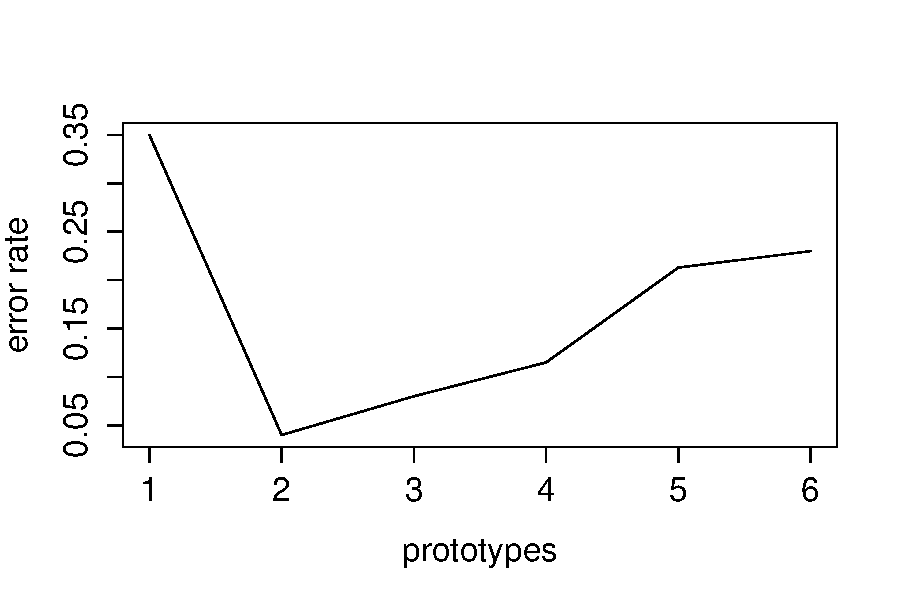
\includegraphics[width=0.8\textwidth]{1.pdf}
	\caption{Error rates versus number of prototypes}
\end{figure}

Then we use $5$-fold cross validation to further examine the relationship between the classification error rate and the number of prototypes. The results are summarized in Table \ref{tab2}:
\begin{table}[htbp]
	\begin{center}
		\caption{\label{tab2} Classification error rate versus number of prototypes using cross validation}
		\begin{tabular}{c|cccccc}
			\hline
			Number of prototypes&1 &2 &3 &4&5&6 \\
			\hline
			Error Rates &0.35 &0.0424 &0.083&0.116&0.213&0.227  \\
			\hline
		\end{tabular}
	\end{center}
\end{table}
From Table \ref{tab2}, we know that the optimal choice of the number of the prototypes should be $2$.
\section{K-means with dimension reduction}
In this section, we examined the effect of dimension reduction on classification. We first standardized the design matrix and did eigen decomposition of the covariance matrix of the standardized design matrix. The ratio of each principle component explain the total variance is summarized in Table \ref{tab3}.
\begin{table}[htbp]
	\begin{center}

		\caption{\label{tab3} Contributions of each component}
		\begin{tabular}{c|cccccccccc}
			\hline
			Ratio &0.655& 0.086& 0.060& 0.051& 0.042& 0.034& 0.033& 0.029& 0.010 \\
			\hline
		\end{tabular}
	\end{center}
\end{table}
We decided to use the first two components which account for $74$\% of the total variance. Then the design matrix only has two columns. By repeating the process described in section 2, the classification error rates are summarized in Table \ref{tab4}.
\begin{table}[htbp]
	\begin{center}
		\caption{\label{tab4} Classification error rate using dimension reduction}
		\begin{tabular}{c|cccccc}
			\hline
			Number of prototypes&1 &2 &3 &4&5&6 \\
			\hline
			Error Rates &0.35 &0.041 &0.146&0202&0.2225&0.197  \\
			\hline
		\end{tabular}
	\end{center}
\end{table}
Thus, for the data set we used in the project, dimension reduction does not improve the classification error rate. Maybe it is because the two classes of samples in the breast cancer data set are well separated. The relationship between error rates and number of the prototypes is shown in Figure~\ref{fig:kmeans1}.
\begin{figure}
	\centering
	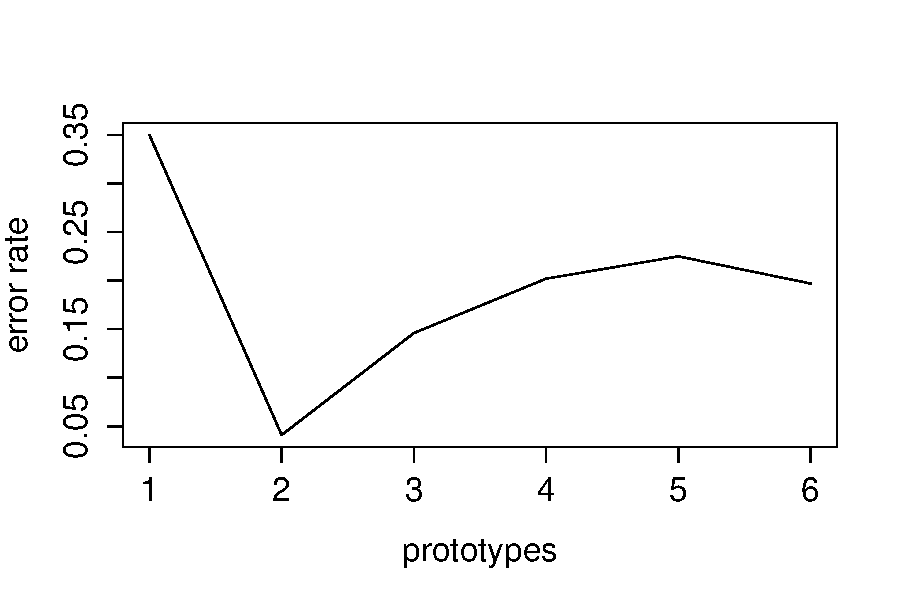
\includegraphics[width=0.8\textwidth]{7.pdf}
	\caption{Error rates versus number of prototypes}
	\label{fig:kmeans1}
\end{figure}

\section{$k$-nearest neighbor classification}

We used the $k$-nearest neighbor method to classify the data as well. We randomly split the data into equal-sized training and test sets, and we also tried leave-one-out cross-validation as well. Figure~\ref{fig:knn1} compares the error rates for each of these methods for $k = 1, \dots, 15$ neighbors.

As the figure shows, $k=3$ performed the best on the split data, and $k=6$ was best according to cross-validation. It appears that cross-validation performed better over a wider range of values of $k$; anything from $k=5$ to $9$ had comparably low error rates, and they were all lower than most error rates using the split data set. For both methods, though, the error rates were highest at $k=1$, then dropped sharply before steadily rising again as $k$ increased.

\begin{figure}
	\centering
	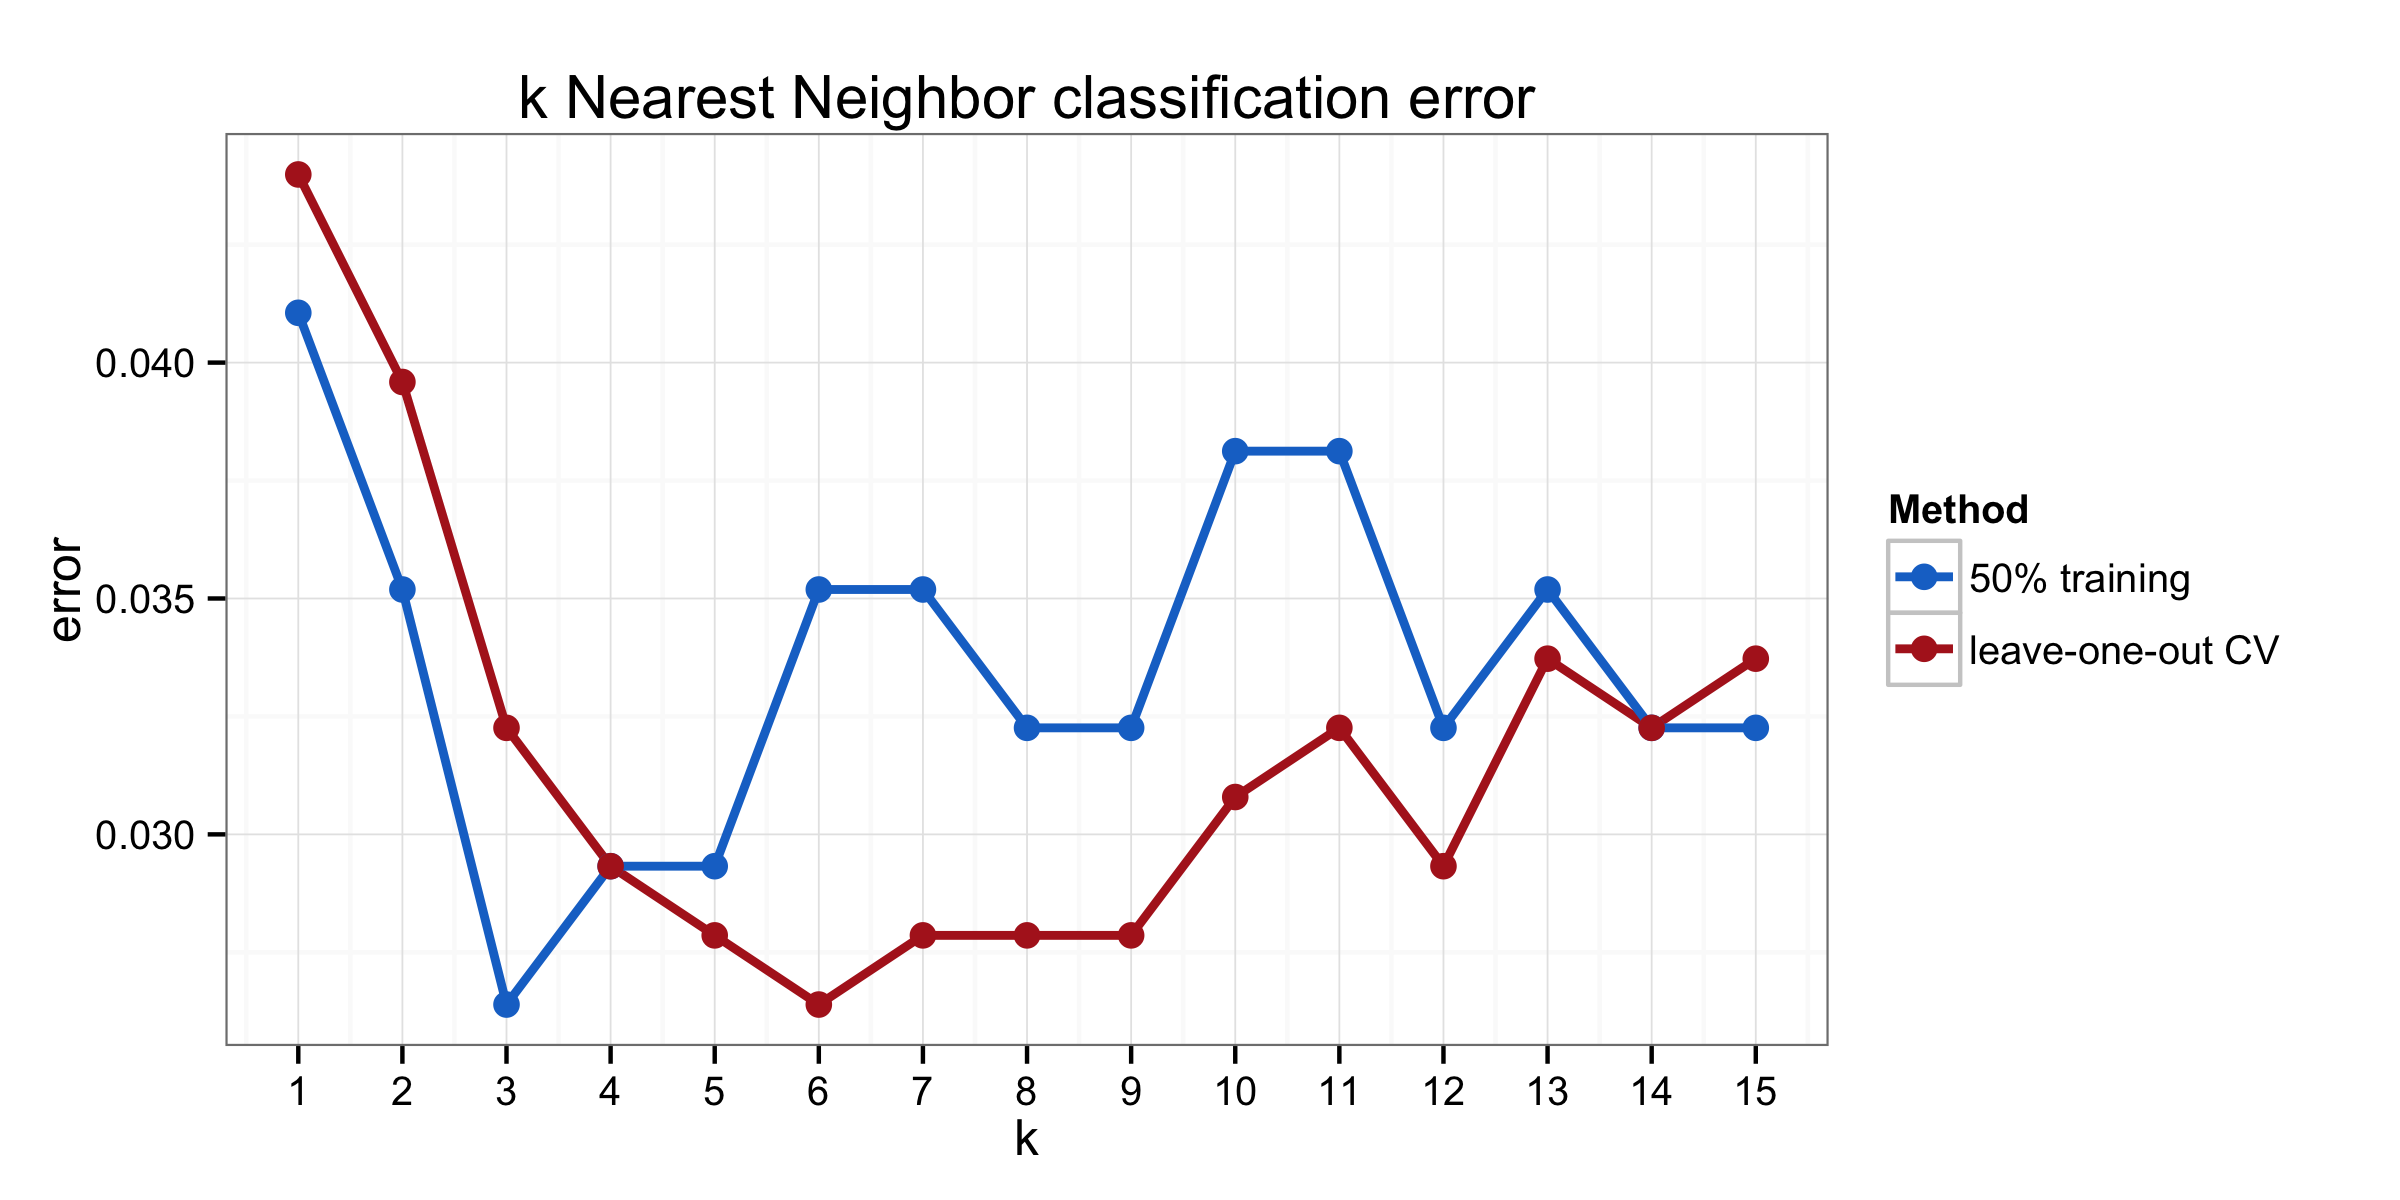
\includegraphics[width=0.8\textwidth]{knn1.png}
	\caption{$k$ nearest neighbor classification results.}
	\label{fig:knn1}
\end{figure}

\section{Unsupervised clustering}
In this section, we try several different numbers of clusters for the data set. We use $2$ to $6$ centroids and all the results are shown in Figure~\ref{fig:kcenter1}.
\begin{figure}
	\centering
	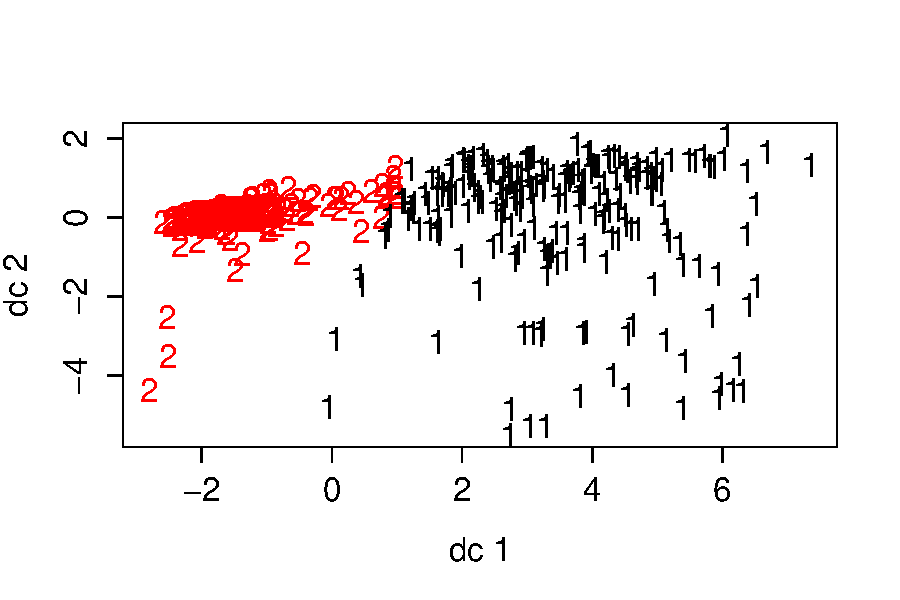
\includegraphics[width=0.4\textwidth]{2.pdf}
	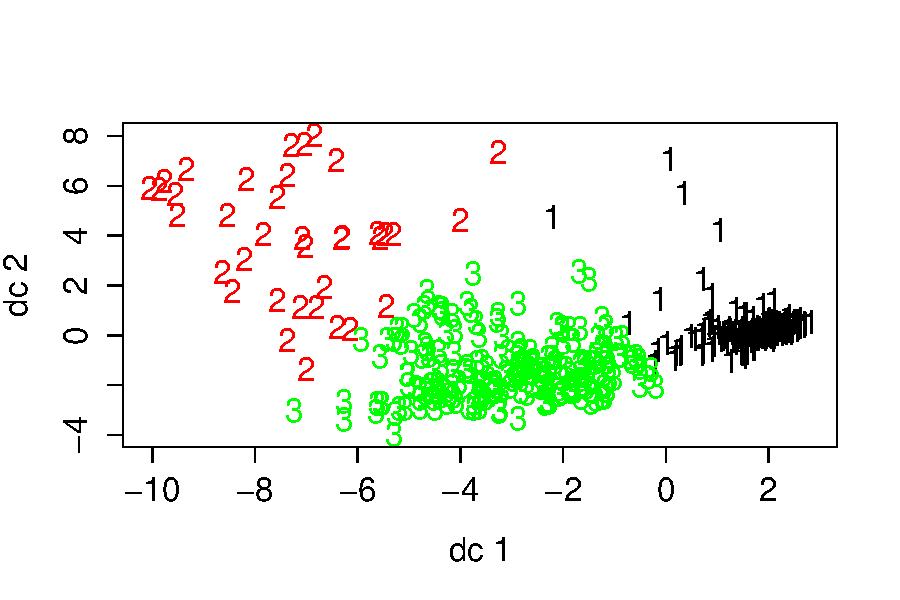
\includegraphics[width=0.4\textwidth]{3.pdf}
	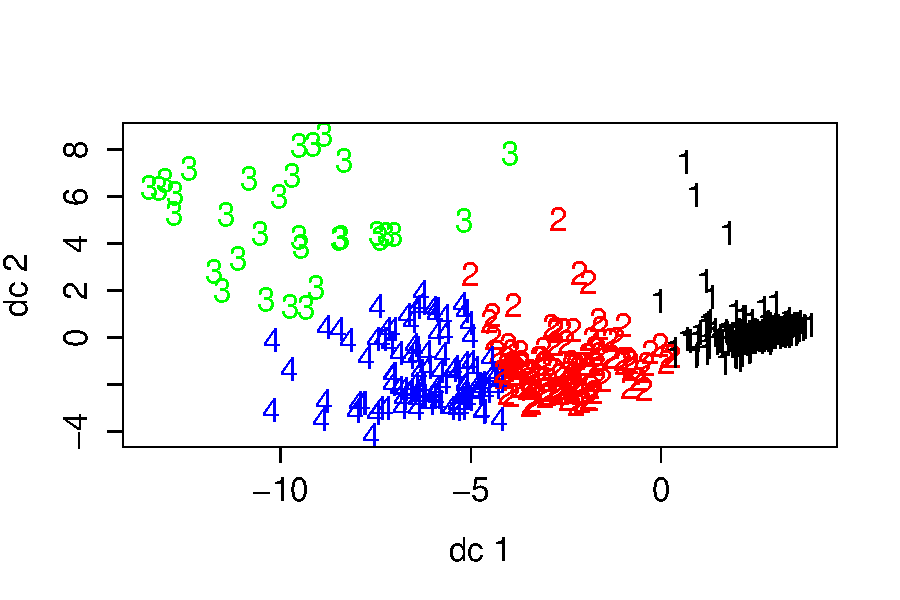
\includegraphics[width=0.4\textwidth]{4.pdf}
	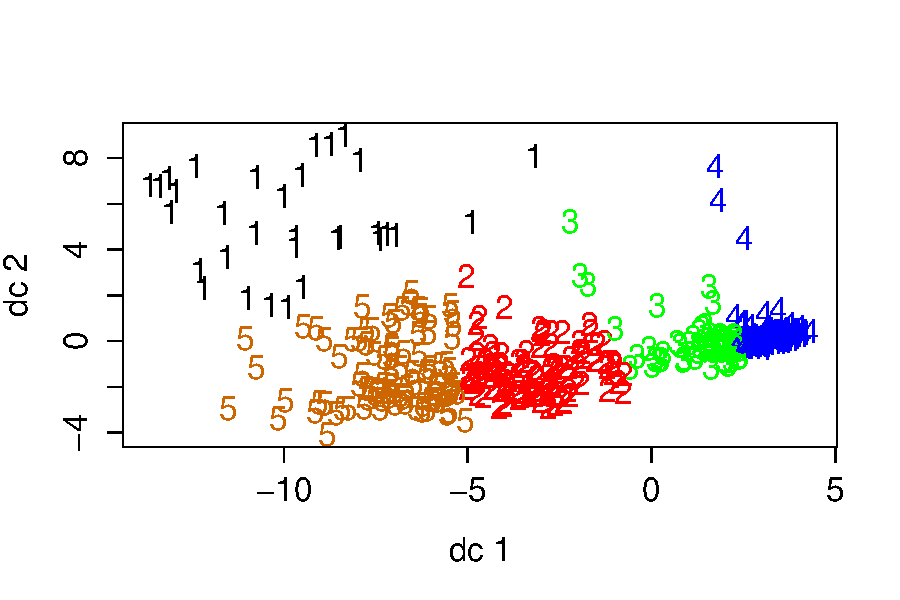
\includegraphics[width=0.4\textwidth]{5.pdf}
	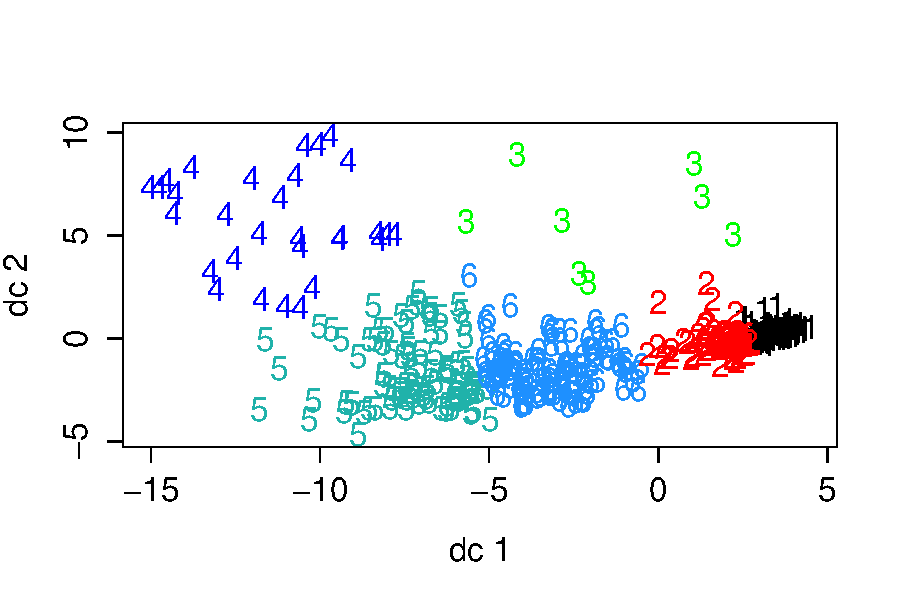
\includegraphics[width=0.4\textwidth]{6.pdf}
	\caption{Unsupervised clustering results}
	\label{fig:kcenter1}
\end{figure}



\section{K-Center}

In k-center clustering we are seeking minimize the maximum inter-cluster distance. In a plane, were seeking to find the smallest radius such that all point in the fix space are contained in k circles with radius r.  The k-center problem is NP-hard and the algorithm proposed by Gonzalez guarantees to produce clustering whose cost is at most twice the optimal.

\subsection{Unsupervised clustering using K-center}

In this section we perform unsupervised clustering by dividing the data into $2$ to $6$ clusters and the result is shown in Figure~\ref{fig:kcenter2}.

\begin{figure}
	\centering
	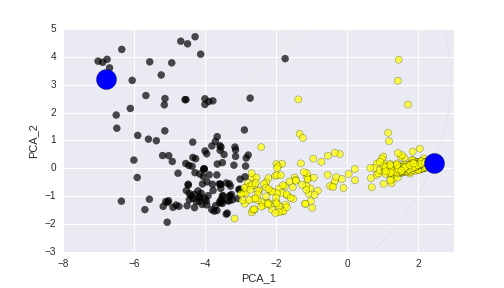
\includegraphics[width=0.4\textwidth]{m1.png}
	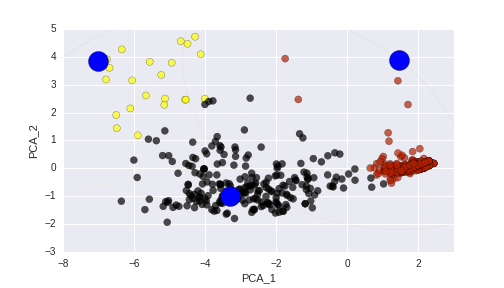
\includegraphics[width=0.4\textwidth]{m2.png}
	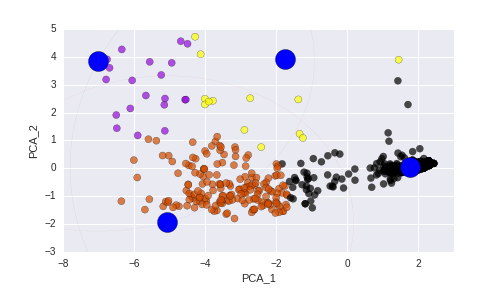
\includegraphics[width=0.4\textwidth]{m3.png}
	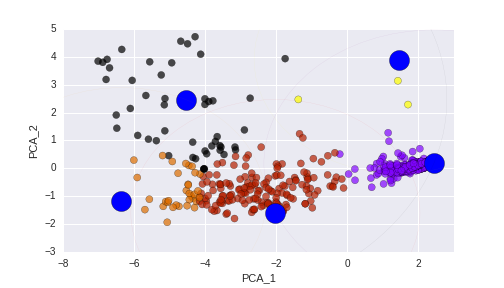
\includegraphics[width=0.4\textwidth]{m4.png}
	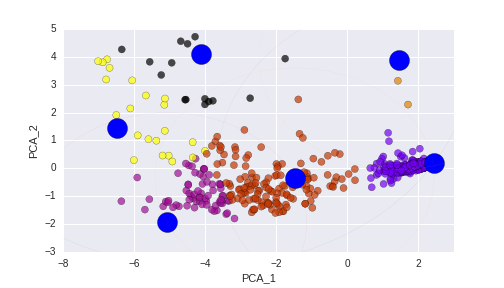
\includegraphics[width=0.4\textwidth]{m5.png}
	\caption{K-center unsupervised clustering results}
	\label{fig:kcenter2}
\end{figure}



\end{document}
